\documentclass[journal]{IEEEtran}
\usepackage{amsmath}
\usepackage{graphicx}
\usepackage{cite}
\usepackage[hidelinks]{hyperref}
\title{Segmentation-Based Screening of Potential Helicopter Landing Areas in Bhadra, Karnataka}
\author{Research manuscript draft}
\begin{document}
\maketitle
\begin{abstract}
We evaluate a geospatial workflow for proposing potential helicopter landing footprints from image segmentation in Bhadra, Karnataka, India. The Helicopter Emergency Landing Place Suggestion System (HELPS) composes Segment Anything ViT-H mask proposals and image-edge regions, then applies an existing random forest and region rules to assign land-cover labels. From 112,283 source regions labelled as low vegetation or bare and sparse ground, the workflow contracts polygons inward, subtracts exclusion and overlap masks, and applies minimum footprint geometry and complete valid slope support at or below 12 degrees on a 30 m terrain grid. The audited result comprises 2,810 segmentation-derived additions from 2,569 contributing source regions, covering 11.543428 square kilometres. The highest admitted grid-cell slope was 11.971163 degrees. The imagery acquisition date is unknown and the study has no independent ground truth. The results quantify how the rules screened the mapped evidence. They cannot establish detection accuracy or physical landing suitability.
\end{abstract}
\begin{IEEEkeywords}
Aerial imagery, geographic information systems, helicopter landing areas, image segmentation, random forests, terrain screening.
\end{IEEEkeywords}

\section{Introduction}
\IEEEPARstart{U}{nprepared} landing areas vary in usable extent, surface condition, terrain slope, and nearby hazards. Operational decisions require reconnaissance and aircraft-specific procedures \cite{faa}. HELPS supports the earlier map-based task of identifying footprints that warrant examination. In this study a qualifying footprint is a mapped polygon that satisfies specified data and rule checks. A segmentation-derived addition is a qualifying footprint whose lineage starts in a classified image segment, after removing overlap with polygons already admitted to the proposal.

The contribution is a traceable case study of a segmentation pipeline and subsequent terrain screening across Bhadra. We report the source label inventory, the qualification rules, and the count and extent of the additions. Retaining the source label and the identifier of each contributing region lets the analysis distinguish source-region outcomes from resulting polygon counts. The case study addresses feasibility and auditability. The absence of independent ground truth prevents estimates of omission, commission, and operational safety.

\section{Related Work}
Scherer \emph{et al.} assessed geometry and approach feasibility with onboard lidar and demonstrated autonomous landings on a full-scale helicopter \cite{scherer}. HELPS uses previously acquired map evidence for screening, which offers a different spatial and temporal view of the terrain. Erskine \emph{et al.} compared surveyed helicopter landing zones with estimates from land-cover and elevation inputs sampled at 1--30 m. Feature scale and local geography affected boundary accuracy \cite{erskine}. Their surveyed footprints supplied reference evidence that is unavailable in the Bhadra study.

Segment Anything (SAM) supports promptable and automatic mask generation \cite{sam}. Geospatial adaptations such as SamGeo have demonstrated its use with georeferenced imagery \cite{samgeo}. In the Bhadra pipeline, SAM contributes mask boundaries, while an existing random forest based on Breiman's method and context rules supply semantic labels \cite{neha,breiman}. The assessment considers the combined classification and screening workflow. It does not isolate the contribution of SAM relative to the other boundary sources.

\section{Study Area and Inputs}
\subsection{Imagery and classified vectors}
The Bhadra boundary covers approximately 1,107.33 square kilometres. The project sampled Esri World Imagery in overlapping windows, preferring zoom 19 and falling back to zoom 18. It projected the working grid to WGS 84 / UTM zone 43N (EPSG:32643) at approximately 0.485 m spacing. This value is the processing-grid spacing. Native imagery resolution, acquisition date, and whether all tiles share a common acquisition date remain unverified.

The final classified GeoPackage contains 761,031 polygons across 1,861 recorded batch identifiers. Its two grouped layers contain 112,283 potentially open regions and 648,748 other regions. The open layer contains 37,556 low-vegetation polygons and 74,727 bare or sparse ground polygons. The other layer retains the original labels for water, woody vegetation, roofs, industrial structures, roads, and uncertainty. Counts and class areas describe the supplied labels. Batch count alone does not establish regional coverage quality.

\subsection{Terrain and context}
The screening uses the saved 30 m FABDEM grid. FABDEM was designed to reduce vegetation and building height biases in the Copernicus elevation product \cite{fabdem}. Mapped exclusions and reviewed rejects provide additional context, with their coverage limits retained. The linked knowledge package carries a 1 June 2026 context date. The acquisition date of the segmented imagery remains unknown.

\section{Method}
\subsection{Segmentation and region labels}
The Bhadra producer uses pretrained SAM ViT-H in automatic mode on windows with a halo for image context. A composition stage reconciles overlapping masks and accepted reference footprints. It fills remaining areas with graph-based image-edge regions following Felzenszwalb and Huttenlocher \cite{felz}, cleans small fragments, and clips the output to each batch core. The resulting partition therefore includes SAM, reference, and edge-derived boundaries. Seam-adjacent features can remain split.

An existing scene-specific forest predicts per-pixel classes from 16 colour, texture, and road-context features. Region voting and confidence and context rules assign the final labels. Some roofs and other engineered features use accepted references or review rules. Region uncertainty stays explicit. The seed categories are class 3 (crops, grass, and low vegetation) and class 4 (bare soil, rock, and sparse ground). Neither class establishes surface height, firmness, or clearance. Figure~\ref{fig:detail} shows the label partition and the retained footprints for one detail window.
\begin{figure*}[t]
\centering
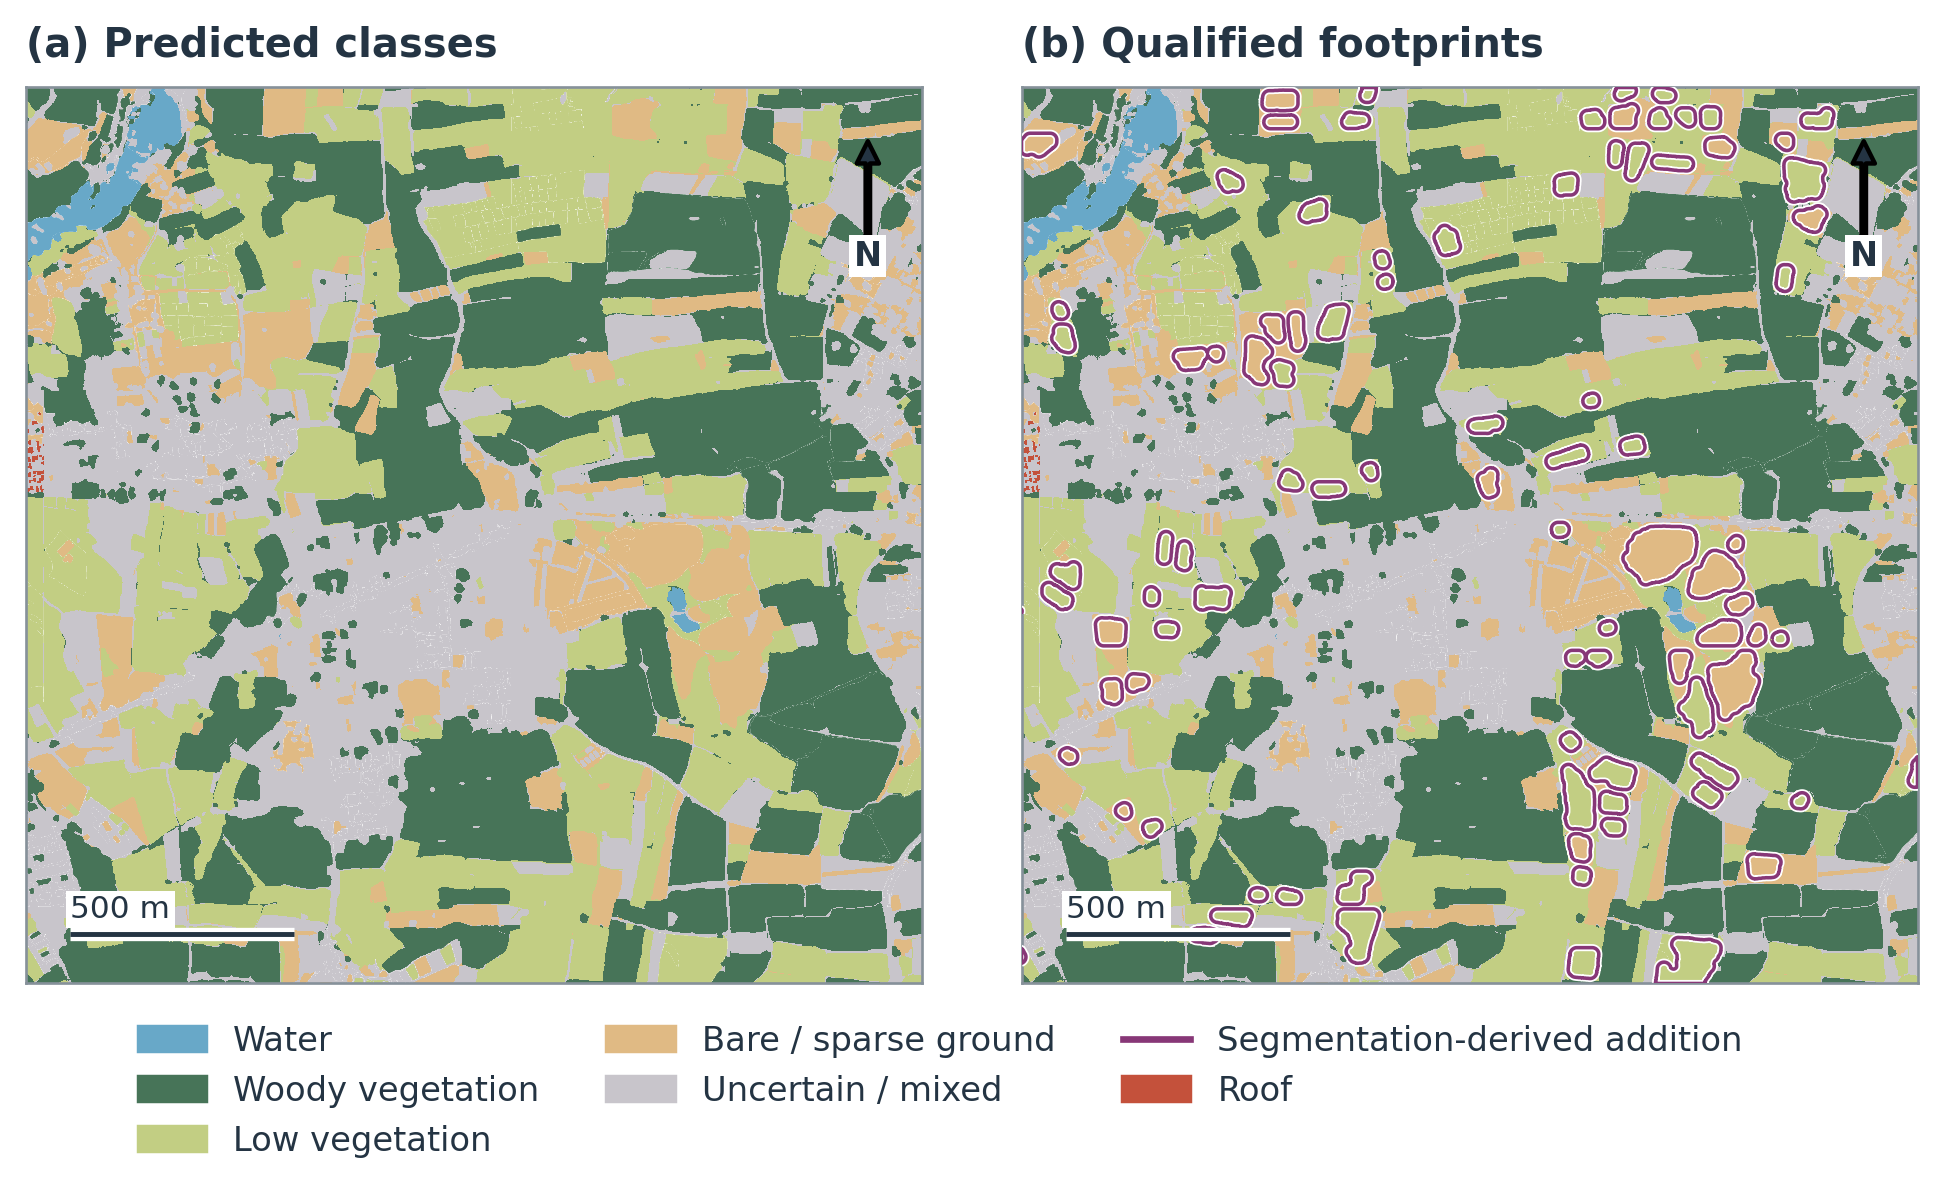
\includegraphics[width=\textwidth]{figures/bhadra-segmentation.png}
\caption{Bhadra segmentation and qualification in a 2 km square detail window. Panel (a) shows predicted classes. Panel (b) overlays the segmentation-derived additions outlined in purple. Both panels are redrawn from saved polygons in EPSG:32643. The detail window location is marked in Fig.~\ref{fig:additions}.}
\label{fig:detail}
\end{figure*}

\subsection{Spatial filtering and geometry}
Let $P_i$ be a source open polygon, $B$ the study boundary, $E$ the applicable exclusions, and $A_i$ the footprints already admitted when $P_i$ is processed. The initial contraction $P_i^{(-5)}$ offsets the boundary inward by 5 m. The proposal stage checks geometry and slope on contracted components before subtracting exclusions and overlaps. For the subset that passes those preliminary gates, the remaining geometry is computed as
\begin{equation}
Q_i = (P_i^{(-5)} \cap B) \setminus (E \cup A_i).
\label{eq:filter}
\end{equation}
The mask $E$ combines the applicable mapped exclusions and reviewed rejects with the vision classes outside 3 and 4. Uncertain class 8 is withheld by policy, even though uncertainty does not establish a physical obstruction. Subtracting $A_i$ prevents a proposed footprint from duplicating existing admitted polygons or earlier additions.

The remaining pieces undergo the shared geometry checks. They must have area at least $900\,\mathrm{m}^2$, both dimensions of the minimum rotated rectangle at least $30\,\mathrm{m}$, and a maximum inscribed clear diameter of at least $30\,\mathrm{m}$. A 15 m erosion and dilation opening removes narrow connections and is intersected with the input geometry. Geometry is rechecked on the surviving pieces. Clear diameter refers to mapped two-dimensional containment.

\subsection{Terrain and lineage checks}
Slope is estimated from a Horn $3 \times 3$ derivative on the 30 m metric grid \cite{horn}. For a candidate footprint, every grid cell with a positive-area intersection must be valid. The maximum of the intersecting cell slopes must be at most $12^\circ$. The check is performed again after footprint filtering. This threshold was the Bhadra producer's terrain screen. Aircraft limits and approach considerations require separate evidence.

Each output retains the source region key, class, batch identifier, and the unknown imagery date. The independent software audit checked polygon validity, containment within the contracted source, overlap against exclusions and other accepted polygons, slope and valid DEM support, and package relationships. These checks verify the implementation against supplied inputs and rules. Field verification was outside their scope.

\section{Results}
\subsection{Source-region decisions and footprint yield}
Of 112,283 source open regions, 2,569 contributed at least one qualifying footprint. They produced 2,810 additions after splitting and screening. The audit assigned 107,864 source regions the contracted-geometry rejection reason and 1,850 the slope-above-limit reason. These are recorded terminal reasons. Sequential filtering and polygons with multiple components mean they are not a count of every reason each source could fail.

The additions cover 11.543428 square kilometres. Table~\ref{tab:class} breaks down the count and area by the original source label. The median footprint area was 2,345.55 square metres, with an interquartile range from 1,502.82 to 4,010.65 square metres. The median maximum cell slope was 3.04 degrees, and the highest was 11.971163 degrees. Figure~\ref{fig:additions} shows locations and the maximum-slope distribution. The model's source labels have not been independently checked against ground conditions.
\begin{table}[t]
\caption{Segmentation-derived additions by source class}
\label{tab:class}
\centering
\begin{tabular}{lrr}
\hline
Source label & Footprints & Area (km$^2$) \\
\hline
Low vegetation (3) & 1508 & 5.335627 \\
Bare / sparse ground (4) & 1302 & 6.207801 \\
Total & 2810 & 11.543428 \\
\hline
\end{tabular}
\end{table}

The independent software audit found all additions inside their 5 m contracted source polygons and recorded full DEM support to numerical tolerance. The package was subsequently selected following explicit review. It also contains separately tracked retained fragments. The counts, areas, and slope statistics in this paper refer only to the segmentation-derived additions.
\begin{figure*}[t]
\centering
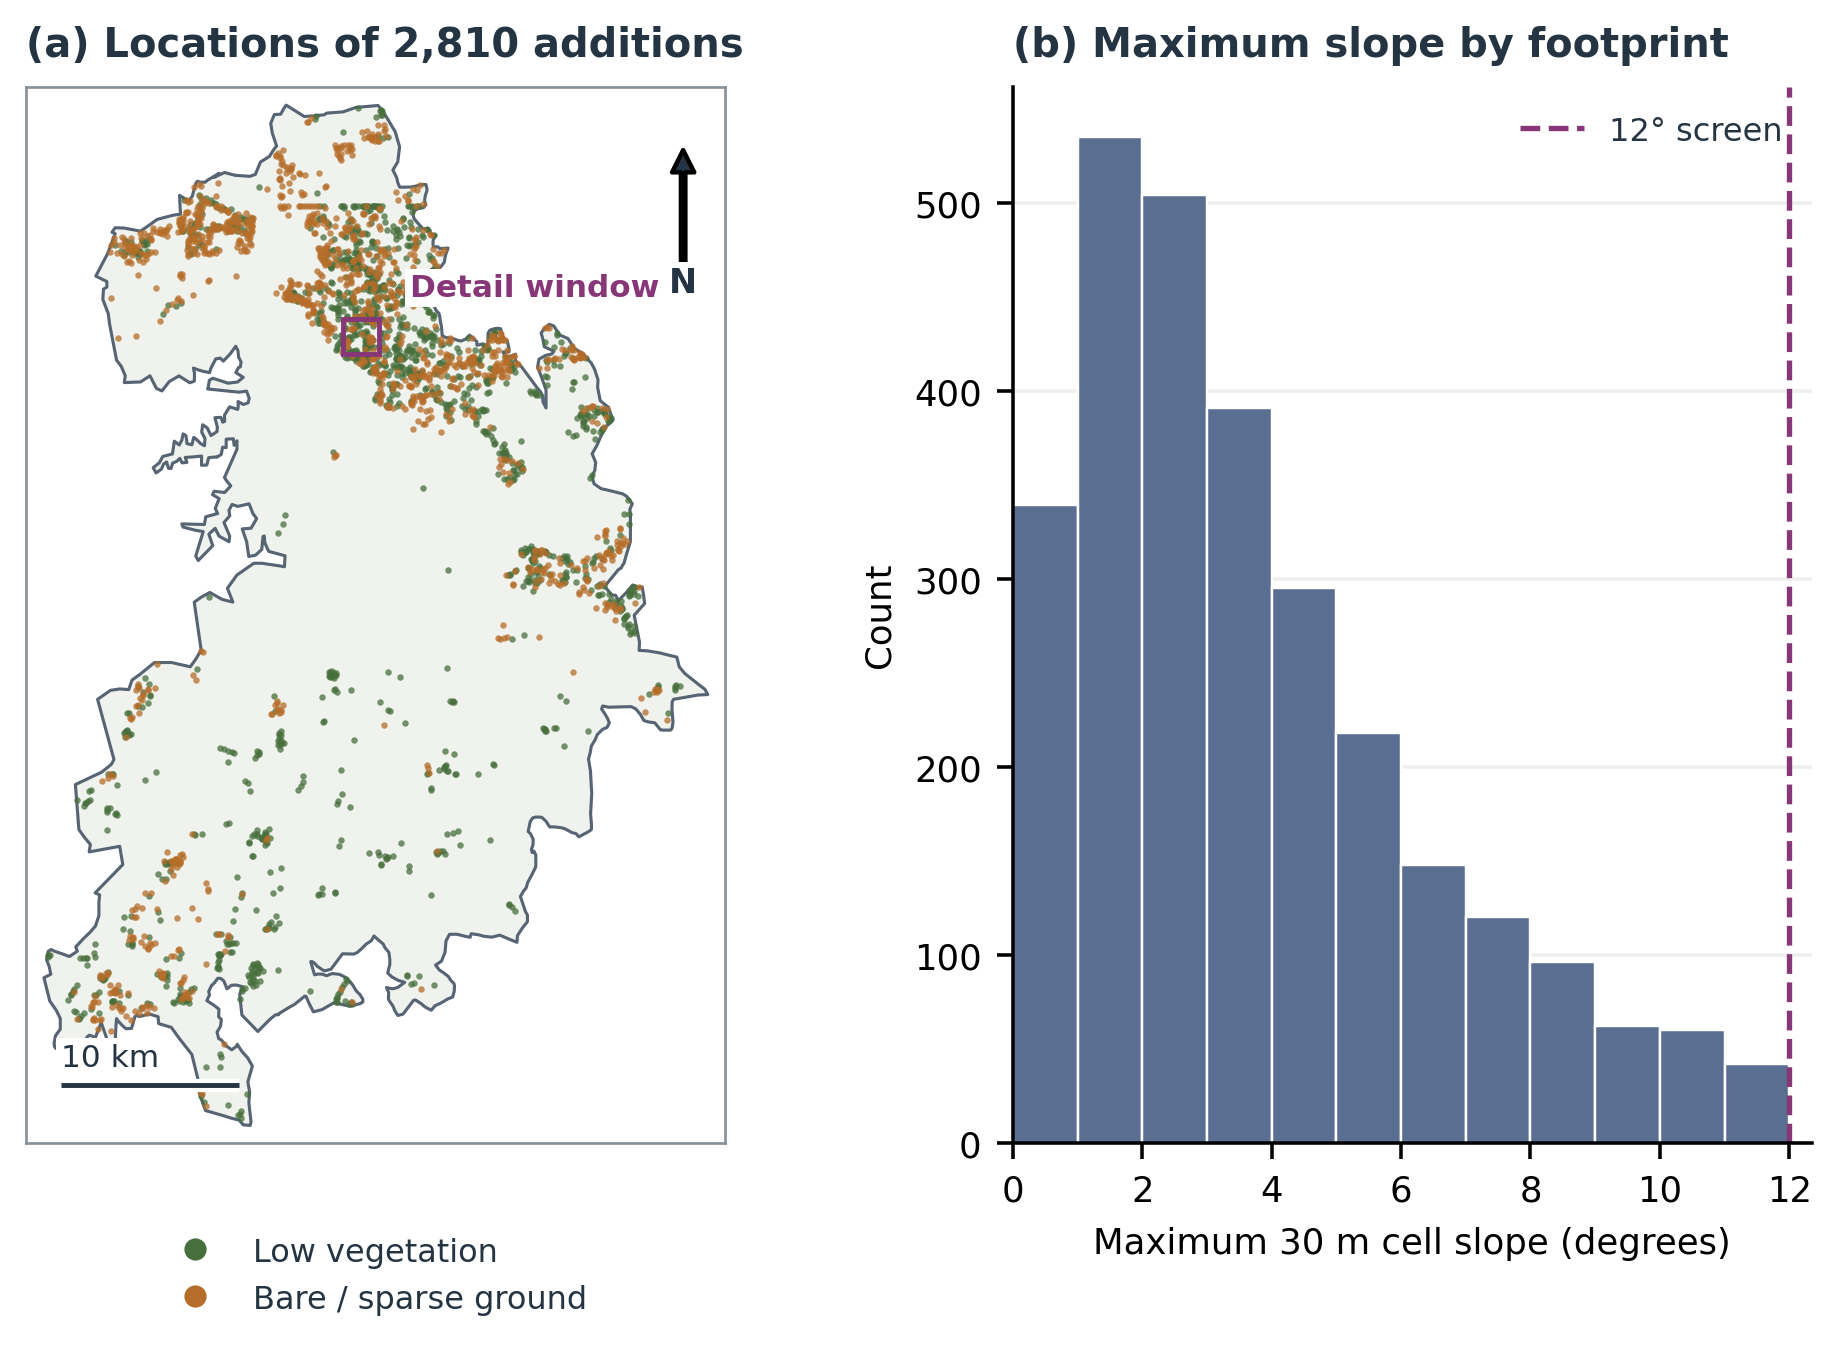
\includegraphics[width=\textwidth]{figures/bhadra-additions.png}
\caption{Spatial and slope summaries for the 2,810 segmentation-derived additions. Panel (a) plots one interior point per footprint, grouped by source class, and marks the detail window shown in Fig.~\ref{fig:detail}. Panel (b) plots each footprint's highest intersecting 30 m slope cell and the 12 degree qualification threshold.}
\label{fig:additions}
\end{figure*}

\section{Limitations and Validation Design}
The study has no independent ground truth for land-cover polygons, obstacles, or feasible helicopter landing footprints. Model labels and reference layers used during classification cannot serve as an independent benchmark. Software verification confirms consistency with the supplied polygons and terrain raster. It leaves false positives, omissions, and geographic generalization unmeasured. Image age and capture-date variation also remain unknown. Small hazards such as wires and local slope changes may be missed. The measured grid and footprint diameter cannot establish ground bearing capacity or approach clearance.

A follow-up should sample spatially separated blocks and use date-matched reference imagery interpreted independently of the model and its priors. Stratification should cover both predicted seed classes, uncertainty, rejected regions, and relevant terrain types. Area-adjusted confusion estimates and confidence intervals should reflect the sampling design \cite{olofsson}. Visible opening boundaries can be evaluated with polygon intersection-over-union and precision and recall. Reference sampling should include output-free areas to estimate omissions. A separate field or higher-resolution 3-D study is needed to evaluate obstacles, local slope, and physical suitability.

\section{Conclusion}
The Bhadra workflow translated segmentation and land-cover labels into 2,810 traceable terrain footprints that passed specified geometry and 30 m slope checks. Independent field or reference validation is needed before interpreting these footprints as accurately detected openings or physically suitable sites.

\section*{Data and Reproducibility}
The archived classified and qualification GeoPackages, decisions, and verification reports are indexed in the accompanying reproduction notes. The maps are original thematic renders of the saved vectors.
\begin{thebibliography}{11}
\bibitem{faa}
Federal Aviation Administration, \emph{Helicopter Flying Handbook}, FAA-H-8083-21B, 2019, chs. 5, 10--11. [Online]. Available: \url{https://www.faa.gov/regulations_policies/handbooks_manuals/aviation/helicopter_flying_handbook}
\bibitem{scherer}
S. Scherer, L. Chamberlain, and S. Singh, "Autonomous landing at unprepared sites by a full-scale helicopter," \emph{Robot. Auton. Syst.}, vol. 60, no. 12, pp. 1545--1562, Dec. 2012, doi: \href{https://doi.org/10.1016/j.robot.2012.09.004}{10.1016/j.robot.2012.09.004}.
\bibitem{erskine}
J. Erskine, C. Oxendine, W. Wright, M. O'Banion, and A. Philips, "Evaluating the relationship between data resolution and the accuracy of identified helicopter landing zones (HLZs)," \emph{Appl. Geogr.}, vol. 139, Feb. 2022, Art. no. 102652, doi: \href{https://doi.org/10.1016/j.apgeog.2022.102652}{10.1016/j.apgeog.2022.102652}.
\bibitem{sam}
A. Kirillov \emph{et al.}, "Segment anything," in \emph{Proc. IEEE/CVF Int. Conf. Comput. Vis. (ICCV)}, 2023, pp. 4015--4026, doi: \href{https://doi.org/10.1109/ICCV51070.2023.00371}{10.1109/ICCV51070.2023.00371}.
\bibitem{samgeo}
Q. Wu and L. P. Osco, "samgeo: A Python package for segmenting geospatial data with the Segment Anything Model (SAM)," \emph{J. Open Source Softw.}, vol. 8, no. 89, Sep. 2023, Art. no. 5663, doi: \href{https://doi.org/10.21105/joss.05663}{10.21105/joss.05663}.
\bibitem{neha}
Nehareddy1234, \emph{cv\_ai\_helps}, GitHub software repository, reviewed revision 47843a288f195e1bbb1eb2df7481d7ec255c9eb1. [Online]. \href{https://github.com/Nehareddy1234/cv_ai_helps/tree/47843a288f195e1bbb1eb2df7481d7ec255c9eb1}{Pinned implementation}.
\bibitem{breiman}
L. Breiman, "Random forests," \emph{Mach. Learn.}, vol. 45, no. 1, pp. 5--32, Oct. 2001, doi: \href{https://doi.org/10.1023/A:1010933404324}{10.1023/A:1010933404324}.
\bibitem{fabdem}
L. Hawker \emph{et al.}, "A 30 m global map of elevation with forests and buildings removed," \emph{Environ. Res. Lett.}, vol. 17, no. 2, 2022, Art. no. 024016, doi: \href{https://doi.org/10.1088/1748-9326/ac4d4f}{10.1088/1748-9326/ac4d4f}.
\bibitem{felz}
P. F. Felzenszwalb and D. P. Huttenlocher, "Efficient graph-based image segmentation," \emph{Int. J. Comput. Vis.}, vol. 59, no. 2, pp. 167--181, Sep. 2004, doi: \href{https://doi.org/10.1023/B:VISI.0000022288.19776.77}{10.1023/B:VISI.0000022288.19776.77}.
\bibitem{horn}
B. K. P. Horn, "Hill shading and the reflectance map," \emph{Proc. IEEE}, vol. 69, no. 1, pp. 14--47, Jan. 1981, doi: \href{https://doi.org/10.1109/PROC.1981.11918}{10.1109/PROC.1981.11918}.
\bibitem{olofsson}
P. Olofsson, G. M. Foody, M. Herold, S. V. Stehman, C. E. Woodcock, and M. A. Wulder, "Good practices for estimating area and assessing accuracy of land change," \emph{Remote Sens. Environ.}, vol. 148, pp. 42--57, May 2014, doi: \href{https://doi.org/10.1016/j.rse.2014.02.015}{10.1016/j.rse.2014.02.015}.
\end{thebibliography}
\end{document}
